\documentclass{article}
\usepackage[utf8]{inputenc}
\usepackage[usenames,dvipsnames]{xcolor}
\usepackage{tikz}
\usetikzlibrary{automata, arrows.meta, calc, fit, positioning,shapes}
\usepackage{amsmath,amssymb}

\begin{document}

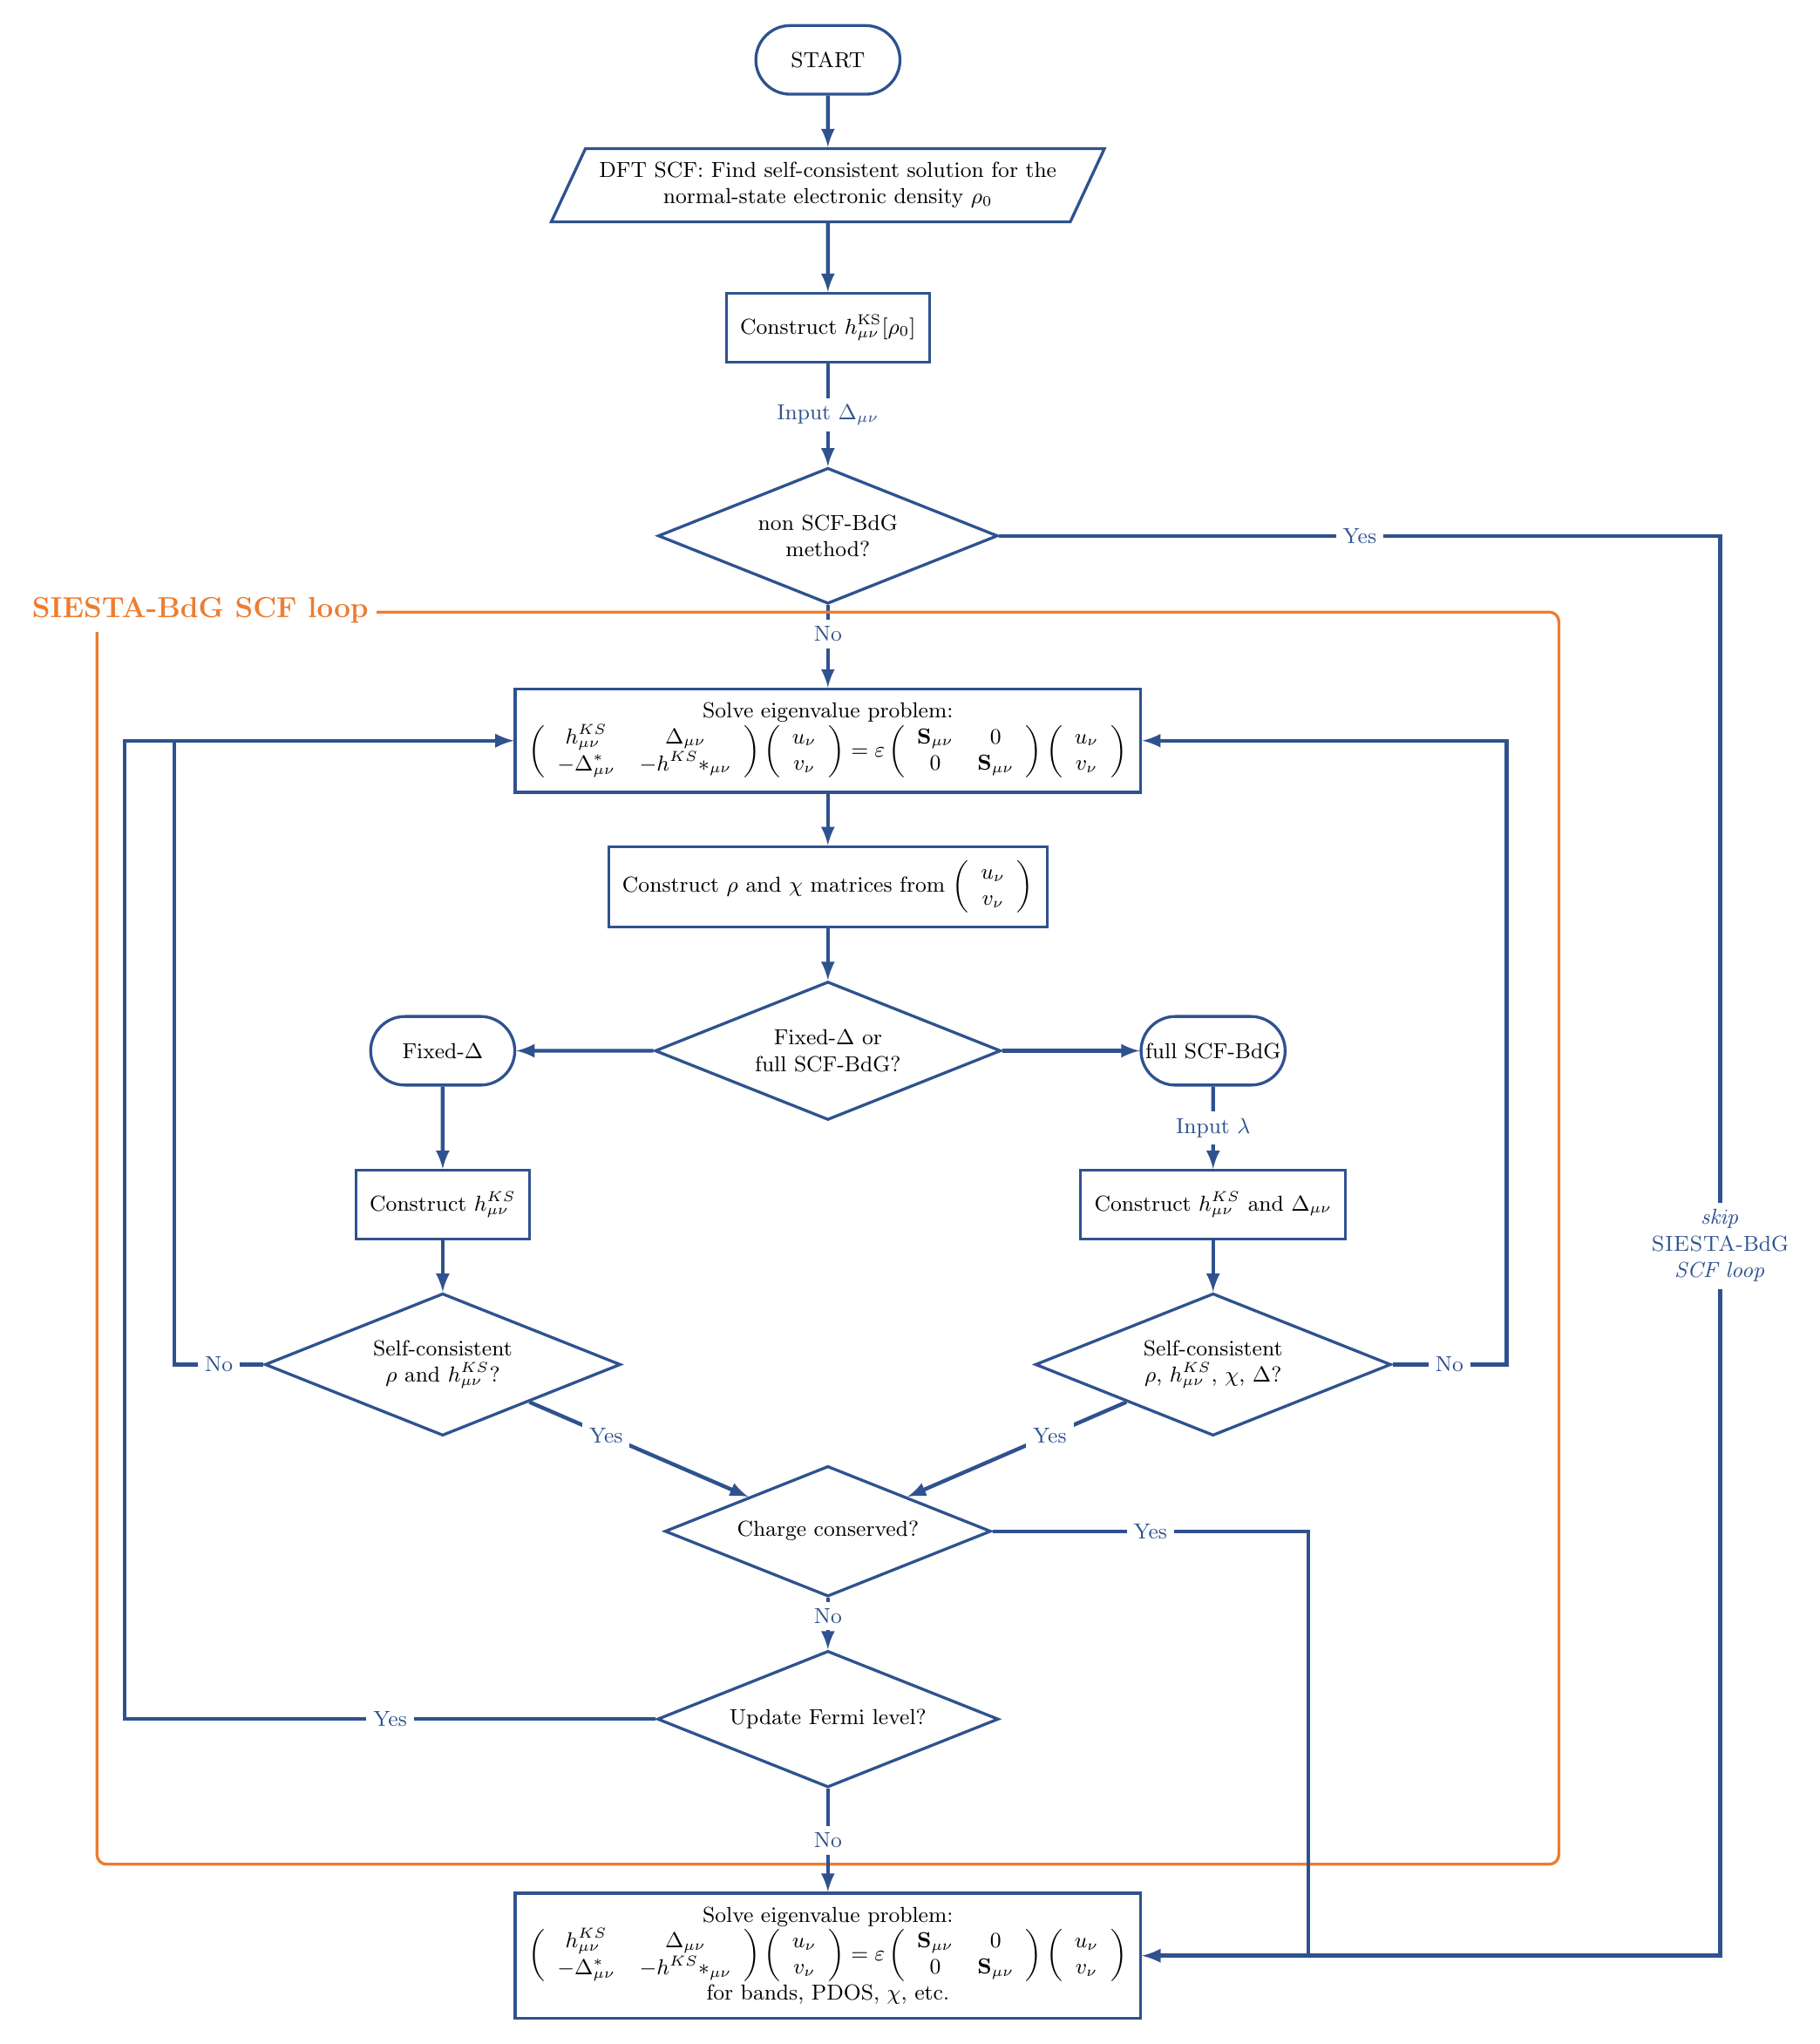
\begin{tikzpicture}[font=\small,align=center,node distance=0.75cm]
    \definecolor{borderColour}{HTML}{2f528f}
    \definecolor{myBlue}{HTML}{4472c4}
    \definecolor{myOrange}{HTML}{ed7d31}
    \definecolor{myGreen}{HTML}{92d050}

    \tikzset{box/.style={
            draw=borderColour, very thick,
            minimum width=2.5cm,
            inner sep=2mm,
            align=center,
            minimum height=1cm}}
    \tikzset{input/.style={
            trapezium,
            trapezium left angle = 65,
            trapezium right angle = 115,
            trapezium stretches}}
    \tikzset{choice/.style={
            diamond,
            aspect=2.5}}
    \tikzset{connect/.style={->, >=latex, ultra thick, borderColour}}

    % Normal part
    \node[box,rounded rectangle] (START) at (0, 0) {START};
    \node[box,input,below=of START] (Rho0) {DFT SCF: Find self-consistent solution for the \\
        normal-state electronic density
        $\rho_0$};  

    \node[box,below=1cm of Rho0] (HofRho) {Construct $h^{\mathrm{KS}}_{\mu\nu}[\rho_0]$};
    \node[box,choice,below=1.5cm of HofRho ] (Oneshot) {non SCF-BdG\\ method?};          

    \node[box,below=1.2cm of Oneshot] (Diag) {Solve eigenvalue problem: \\
        $\left(\begin{array}{cc}
            h^{KS}_{\mu\nu} & \Delta_{\mu\nu}\\
            -\Delta^*_{\mu\nu} & -h^{KS}*_{\mu\nu}
        \end{array}\right)
        \left(\begin{array}{c}
            u_{\nu}\\
            v_{\nu}
        \end{array} \right)
        = \varepsilon \left(\begin{array}{cc}
            \mathbf{S}_{\mu\nu} & 0\\
            0 & \mathbf{S}_{\mu\nu}
        \end{array} \right)
        \left(\begin{array}{c}
            u_{\nu}\\
            v_{\nu}
        \end{array} \right)$};
    \node[box,below=of Diag] (CalcRhoChiFixD0) {Construct $\rho$ and $\chi$ matrices
        from $\left(\begin{array}{c} u_{\nu}\\ v_{\nu}\end{array} \right)$};            
      \node[box,choice,below=of CalcRhoChiFixD0 ] (FixDorFixL) {Fixed-$\Delta$ or \\ full SCF-BdG?};
    % % Fixed-Delta  
    \node[box,rounded rectangle,left=2cm of FixDorFixL] (FixD) {Fixed-$\Delta$};
    \node[box,below=1.2cm of FixD] (CalcHk) {Construct $h^{KS}_{\mu\nu}$};
    \node[box,choice,below=of CalcHk ] (SCFixD) {Self-consistent\\
    $\rho$ and $h^{KS}_{\mu\nu}$?};        
    % % Fixed-Lambda
    \node[box,rounded rectangle,right=2cm of FixDorFixL] (FixL) {full SCF-BdG};
    \node[box,below=1.2cm of FixL] (CalchDFixL) {Construct $h^{KS}_{\mu\nu}$ and $\Delta_{\mu\nu}$};
    \node[box,choice,below=of CalchDFixL] (SCFixL) {Self-consistent\\
    $\rho$, $h^{KS}_{\mu\nu}$, $\chi$, $\Delta$?}; 
    % %Charge
    \node[box,choice,below=5cm of FixDorFixL] (Charge) {Charge conserved?}; 
    \node[box,choice,below=of Charge] (Fermi) {Update Fermi level?}; 
    %Charge        
    %Postprocessing
    \node[box,below=1.5cm of Fermi] (Postprocess) {Solve eigenvalue problem: \\
        $\left(\begin{array}{cc}
            h^{KS}_{\mu\nu} & \Delta_{\mu\nu}\\
            -\Delta^*_{\mu\nu} & -h^{KS}*_{\mu\nu}
        \end{array}\right)
        \left(\begin{array}{c}
            u_{\nu}\\
            v_{\nu}
        \end{array} \right)
        = \varepsilon \left(\begin{array}{cc}
            \mathbf{S}_{\mu\nu} & 0\\
            0 & \mathbf{S}_{\mu\nu}
        \end{array} \right)
        \left(\begin{array}{c}
            u_{\nu}\\
            v_{\nu}
        \end{array} \right)$ \\
        for bands, PDOS, $\chi$, etc.};        

    % %%%%%%%%%%%%%%%%%%%%%%%%%%%%%%%%%%%%%%%%%%%%%%%%%%%%%%%%%%%%%%%
    \draw[connect] (START) -- (Rho0);
    \draw[connect] (Rho0) -- (HofRho);
    \draw[connect] (HofRho) -- (Oneshot) node[pos=0.5,fill=white,inner sep=1mm]{Input $\Delta_{\mu\nu}$};
    \draw[connect] (Oneshot) -- ++(13cm,0)   node[pos=0.5,fill=white,inner sep=1mm]{Yes}  |-node[pos=0.25,fill=white,inner sep=1mm]{\textit{skip} \\ \textsc{SIESTA}-BdG\\\textit{SCF loop}} (Postprocess);
    \draw[connect] (Oneshot) -- (Diag) node[pos=0.35,fill=white,inner sep=1mm]{No};
    \node (SCF) [box,draw=myOrange,rounded corners,inner sep=11mm,fit = (Diag) (SCFixD) (SCFixL)(Fermi),label={[anchor=center,fill=white,font=\large,text=myOrange]135:{\textbf{\textsc{SIESTA}-BdG SCF loop}}},
    minimum width=21.3cm] {};        
    \draw[connect] (Diag) -- (CalcRhoChiFixD0);   
    \draw[connect] (CalcRhoChiFixD0) -- (FixDorFixL);
    \draw[connect] (FixDorFixL) -- (FixD);
    \draw[connect] (FixDorFixL) -- (FixL);
    \draw[connect] (FixD) -- (CalcHk);
    \draw[connect] (CalcHk)-- (SCFixD);
    \draw[connect] (SCFixD) -- (Charge) node[pos=0.35,fill=white,inner sep=1mm]{Yes};
    \draw[connect] (SCFixD) -- ++ (-3.91cm,0) node[pos=0.5,fill=white,inner sep=1mm]{No} |- (Diag);
    \draw[connect] (FixL) -- (CalchDFixL)node[pos=0.5,fill=white,inner sep=1mm]{Input $\lambda$};
    \draw[connect] (CalchDFixL) -- (SCFixL);
    \draw[connect] (SCFixL) -- (Charge)
    node[pos=0.35,fill=white,inner sep=1mm]{Yes};
    \draw[connect] (SCFixL) -- ++ (4.275cm,0) node[pos=0.5,fill=white,inner sep=1mm]{No} |- (Diag);
    \draw[connect] (Charge) -- (Fermi)
    node[pos=0.35,fill=white,inner sep=1mm]{No};
    \draw[connect] (Charge) -- ++(7cm,0) node[pos=0.5,fill=white,inner sep=1mm]{Yes} |- (Postprocess);
    \draw[connect] (Fermi) -- ++(-10.250cm,0) node[pos=0.5,fill=white,inner sep=1mm]{Yes} |- (Diag);
    \draw[connect] (Fermi) -- (Postprocess) node[pos=0.5,fill=white,inner sep=1mm]{No};
    % %%%%%%%%%%%%%%%%%%%%%%%%%%%%%%%%%%%%%%%%%%%%%%%%%%%%%%%%%%%%%%%
\end{tikzpicture}

\end{document}